\documentclass{standalone}
\usepackage{graphicx}	
\usepackage{amssymb, amsmath, amsthm}
\usepackage{color}

\usepackage{tikz}
\usetikzlibrary{intersections, backgrounds, math, arrows.meta}

\definecolor{light}{RGB}{220, 188, 188}
\definecolor{mid}{RGB}{185, 124, 124}
\definecolor{dark}{RGB}{143, 39, 39}
\definecolor{highlight}{RGB}{180, 31, 180}
\definecolor{darkteal}{RGB}{29, 79, 79}
\definecolor{darkolive}{RGB}{97, 123, 45}
\definecolor{gray10}{gray}{0.1}
\definecolor{gray20}{gray}{0.2}
\definecolor{gray30}{gray}{0.3}
\definecolor{gray40}{gray}{0.4}
\definecolor{gray60}{gray}{0.6}
\definecolor{gray70}{gray}{0.7}
\definecolor{gray80}{gray}{0.8}
\definecolor{gray90}{gray}{0.9}
\definecolor{gray95}{gray}{0.95}

\begin{document}

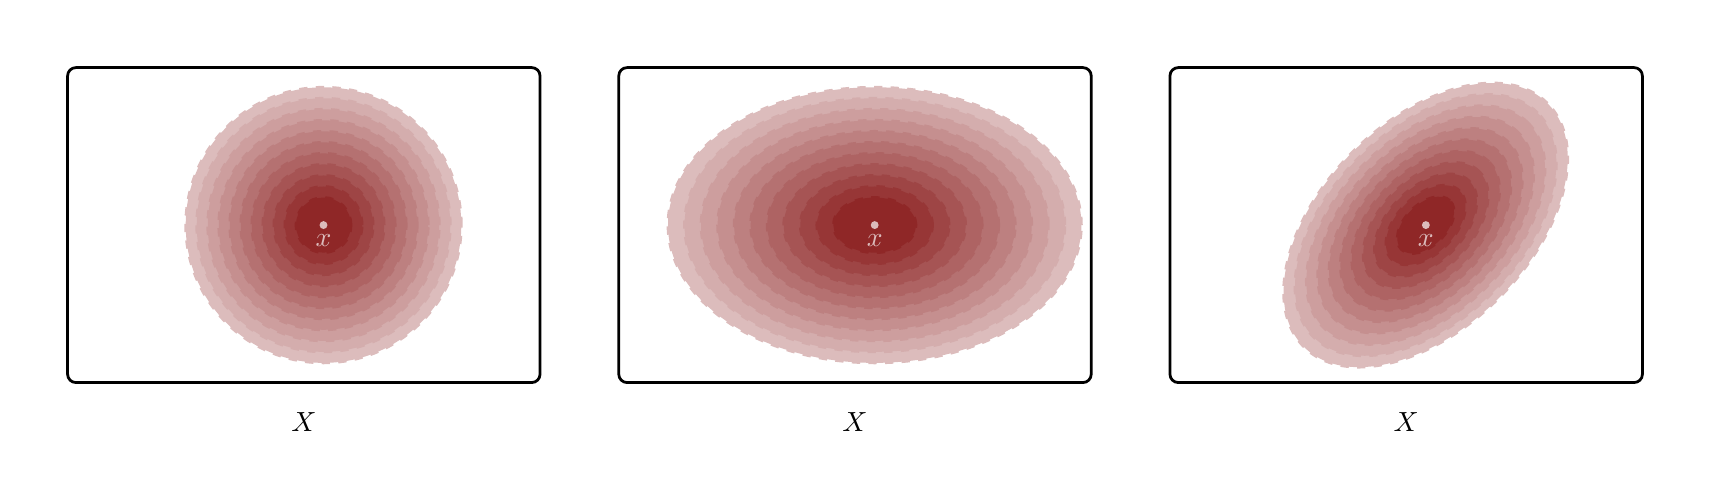
\begin{tikzpicture}[scale=1.0]
  
  \begin{scope}[shift={(0, 0)}]
    \draw[white] (-3.5, -3) rectangle (3.5, 2.5);
  
    \draw[rounded corners=3, color=black, line width=1] (-3, -2) rectangle (3, 2);
    \node at (0, -2.5) { $X$ };
  
    \foreach \n in {0, 1, ..., 10} {
      \pgfmathsetmacro{\r}{1.75 - \n * 1.4 / 10}
      \pgfmathsetmacro{\prop}{100 * \n / 10}
      \colorlet{custom}{dark!\prop!light}; 
      \filldraw[custom, dashed, line width=1] (0.25, 0) circle (\r); 
    }
  
    \fill[light] (0.25, 0) circle (0.05) node[below] { $x$ };
  \end{scope} 

  \begin{scope}[shift={(7, 0)}]
    \draw[white] (-3.5, -3) rectangle (3.5, 2.5);
  
    \draw[rounded corners=3, color=black, line width=1] (-3, -2) rectangle (3, 2);
    \node at (0, -2.5) { $X$ };
  
    \foreach \n in {0, 1, ..., 10} {
      \pgfmathsetmacro{\r}{1.75 - \n * 1.4 / 10}
      \pgfmathsetmacro{\prop}{100 * \n / 10}
      \colorlet{custom}{dark!\prop!light}; 
      \filldraw[custom, dashed, line width=1] (0.25, 0) circle ({1.5 * \r} and \r); 
    }
  
    \fill[light] (0.25, 0) circle (0.05) node[below] { $x$ };
  \end{scope} 
  
  \begin{scope}[shift={(14, 0)}]
    \draw[white] (-3.5, -3) rectangle (3.5, 2.5);
  
    \draw[rounded corners=3, color=black, line width=1] (-3, -2) rectangle (3, 2);
    \node at (0, -2.5) { $X$ };
  
    \foreach \n in {0, 1, ..., 10} {
      \pgfmathsetmacro{\r}{1.75 - \n * 1.4 / 10}
      \pgfmathsetmacro{\prop}{100 * \n / 10}
      \colorlet{custom}{dark!\prop!light}; 
      \filldraw[custom, dashed, line width=1, rotate=45] 
        (0.25 - 0.075, 0 - 0.175) circle ({1.25 * \r} and {0.75 * \r}); 
    }
  
    \fill[light] (0.25, 0) circle (0.05) node[below] { $x$ };
  \end{scope} 
      
\end{tikzpicture}

\end{document}  